\documentclass[11pt]{article} % use larger type; default would be 10pt
\usepackage[utf8]{inputenc} % set input encoding (not needed with XeLaTeX)

%%% BEGIN Article customizations

%%% PAGE LAYOUT
\usepackage{geometry} % to change the page dimensions
\geometry{a4paper} % or letterpaper (US) or a5paper or....
% \geometry{margin=1in} % for example, change the margins to 2 inches all round
\usepackage[parfill]{parskip} % Activate to begin paragraphs with an empty line rather than an indent

%%% FIGURES
\usepackage{graphicx} % support the \includegraphics command and options
\graphicspath{{../FIGURES/FIGURE_PDFS/}}

%%% PACKAGES
\usepackage{booktabs} % for much better looking tables
\usepackage{array} % for better arrays (eg matrices) in maths
\usepackage{paralist} % very flexible & customisable lists (eg. enumerate/itemize, etc.)
\usepackage{verbatim} % adds environment for commenting out blocks of text & for better verbatim
\usepackage{subfig} % make it possible to include more than one captioned figure/table in a single float
% These packages are all incorporated in the memoir class to one degree or another...

%%% HEADERS & FOOTERS
\usepackage{fancyhdr} % This should be set AFTER setting up the page geometry
\pagestyle{fancy} % options: empty , plain , fancy
\renewcommand{\headrulewidth}{0pt} % customise the layout...
\lhead{}\chead{}\rhead{}
\lfoot{}\cfoot{\thepage}\rfoot{}

%%% SECTION TITLE APPEARANCE
\usepackage{sectsty}
\allsectionsfont{\sffamily\mdseries\upshape} % (See the fntguide.pdf for font help)
% (This matches ConTeXt defaults)

%%% ToC (table of contents) APPEARANCE
\usepackage[nottoc,notlof,notlot]{tocbibind} % Put the bibliography in the ToC
\usepackage[titles,subfigure]{tocloft} % Alter the style of the Table of Contents
\renewcommand{\cftsecfont}{\rmfamily\mdseries\upshape}
\renewcommand{\cftsecpagefont}{\rmfamily\mdseries\upshape} % No bold!

%%% END Article customizations

%%% The "real" document content comes below...

\title{Reproducibility of SNP calling in multiple sequencing runs from single tumors}
\author{Dakota Z. Derryberry, Claus O. Wilke, Matthew C. Cowperthwaite} %**ask them about author order, I'm out of it...

\begin{document}
\maketitle

\section{Abstract}

%A) What system are you studying?
We examined 55 technical sequencing replicates of Glioblatoma multiforme (GBM) tumors from The Cancer Genome Atlas (TCGA). %Each replicate included the tumor sequenced once using standard whole exome sequencing with amplification, and once without amplification prior to creating a library.
%B) Why is it important?
In recent years, TCGA \cite{TCGA-GBM} and others in cancer genomics \cite{Parsons} have used large scale sequencing results of many tumors to identify drivers and essential cancer genes using a variety of computational analyses. However, very little is known about the reproducibility of this genomic data and, given the heterogeneity found in tumors, it could be quite low.  
%C) What is your research approach?
Wemeasured the extent of the overlap between two technical sequencing replicates from the same tumor (n=55), to find what proportion of mutations were reliably found between them, using strictly computational means. We further examined whether the raw data was improved or not, as measured by the extent of the overlap, using the SNP calling program SomaticSniper.  
%D) (optional) How is your research different from previous work?
%E) What are the results of your research?
We found that in the raw data, about half of the mutations found in one sequencing run can be found in the second. Interestingly, the size of the overlap varies by two orders of magnitude, between about 50 and 7000. Using a SNP caller, rather than improving the data, removes the overlap completely. This is because overlap is almost entirely composed of LOH, removed automatically by SomaticSniper, and SNPs with only a few reads cvering the alternate allele.
%F) What conclusions can we draw from these results?
We interpret these results to mean that, as expected, sequencing runs of tumors detect many false positives, and the number of these is increased by an amplification step prior to building a library. This tendency aside, the actual number of muations in different tumors of the same type (GBM) may vary by orders of magnitude. Finally, while verificaion of sequencing using PCR remains the gold standard, when SNP-calling using strictly computational means, SNP-callers may actually decrease the quality of results.

\section{Introduction}

A) What is the general field of study?
Glioblastoma multiforme (GBM) is the most common and deadly primary brain tumor, with a median survival of 13.9 months and a 5-year survival of ~5\% \cite{TCGA-GBM-13}. Prognosis for patients with this disease remains poor despite significant research investment, due to the difficulty of surgical resection and the limited number of effective chemoteraputics. Like all cancers, GBM is an evolutionary disease caused by mutations and other alterations to normal glial cell lines. However, following substantial research efforts dedicated to identifying all of the mutations in an individual patient's tumor to try and identify causal variants, few precise causal elationships have been identified. There are likely many related causes for this failure, including but not limited to genomic heterogeneity in tumors, \cite{ValentineD}, the view that "GBM growth is driven by a signaling network with functional redundancy that permits adaptation" \cite{TCGA-GBM-13}, and imperfect computational methods. 
%B) What is the specific question of the research?
In this paper, we are interested in the third. We used technical sequencing replicates from 55 GBM tumors to look at the reproducbility of the raw data using a standard computational pipeline. Assuming that those mutations that appear in each of the technical replicates are true positives, and all others are false positives (which in fact may or may not be true), we want to see what proportion of mutations recovered are ture positives, and whether or not the proportion is increased by SNP-calling methods designed to remove false positives.

%C) Why is (a) and/or (b) important?
The past six years have seen an explosion of data in cancer genomics, an effort led by TCGA, an archive of publicly-available data that includes sequencing of paired tumor-normal samples from a single patient for thousands of tumors. TCGA's glioblastoma dataset alone includes some 580 (and constantly growing) tumor-normal pairs. A varity of researchers in cancer genomics have used this data to discover which genes and pathways are mutated in GBM \cite{pathways}, discover different GBM subtypes \cite{subtypes}, and develop a variety of computational models to find GBM driver mutations \cite{drivers}. Despite this apparent success, most of the relationships discovered, though real, are small effects, and few of these innovations have been successfully translated into clinically useful results and techniques. Several possible factors likely contribute to this effect.
%D) What has previously been done in this area?
[NAME] showed that batch effects have a significant effect on large scale sequencing projects such as TCGA \cite{batch-effects}, and that eliminating this bias without collecting thousands more samples is virtually impossible. While TCGA may eventually do this, eliminating these effects at this time is impossible. Secondly, multiple groups have shown that tumors are highly genetically heterogeneous, and sampling a tumor only once cannot show the entirely of the mutational profile of the tumor \cite{ValentineD} \cite{hetero1} \cite{hetero2}. Third, several groups have shown that epigenetic factors, including methylation \cite{methylation-new}, chromatin remodeling \cite{chromatin}, and micro-RNAs \cite{microRNA}, may significantly effect tumor development and growth. 
%E) How does your research differ?
For all of these reasons, and likley more besides, we know that tumor sequencing is imperfect, and results based on it have to account for a significant amount of noisy data. In this paper, we attempt to look at how much noise (without regard to the theoretical source of it). We take 55 TCGA samples with technical replicates, and look at the similarity of the replicates. 
%F) (end with) a summary of the research described in this paper
We took data from 55 TCGA samples that were sequenced twice, once with the standard WGS protocol, and once with an additional amplification step before library prep, which we call the WGA protocol. We aligned the data and used the SNP-calling program SomaticSniper. Comparing the WGS and WGA results of these 55 samples, we find significant overlap (around 50\%), but as many differences, between technical sequencing replicates of the same sample. As expected, we found that the additional amplification step in the WGA protocol versus the WGS protocol added some mutations to the sample, so that on average these replicates had (i) more mutations, and (ii) a smaller percentage overlap. The number of mutations per sample varied by orders of magnitude, from under 100 to almost 10,000. We expected to see the quality of results (measured by the percentage overlap between technical replicates) decrease with increasing numbers of mutations, but found no correlation. We next looked at standard computational filters meant to increase the quality of the data. We found that to the contrary, employing these filters completely removed the overlap between replicates, and that two filters in particular, one for quality of the alternate allele read and one for loss of heterozygosity, removed most of this data. We conclude that the number of mutations in GBM tumors may be more variable tthan is generally supposed. Further, while nothing will ever beat the biolgical goldstandard of PCR for mutation verification, computational methods need to improve.

\section{Results}

\subsection{Raw data}

% Experiment: size of overlap (figures 1 and 2)
%(a) a brief (one sentence to one paragraph) summary of what you did and why
%(b) a description of what you found carrying out this experiment
For 55 samples, TCGA provides two sets of raw sequence data, one set captured with tthe standard whole exome sequencing methods (WGA) including an amplification of the DNA extracted from the tumor prior to library pred, and one using a protocol for large quantities of DNA that omits this amplification (WGS). For each sample, we analyzed each technical replicate using the same pipeline (see Methods), and then compared the WGA replicate to the WGS replicate, to see the extent of the similarity between the two. We first looked at the similarity between the two replicates, by number of mutations (Figure 1) and percent overlap partcular mutations (Figure 2) between replicates. We found that overall, the number of mutations found in one replicate correlated strongly with the number of mutations found in the other, though as expected the WGA replicate, with the additional amplification step, had slightly more mutations (Figure 1). We found that the overlap between the two samples, caclulated by $WGA \cap WGS/WGS$ for WGS replicates and $WGA \cap WGS/WGA$ for WGA replicates, was mostly between 20-40\% in WGA replicates and mostly between 40-60\% in WGS replicates. As expected the distribution is narrower and taller in the WGS replicates, as a greater percentage of those samples are likley "real" mutations and so present in the overlap (Figure 2).

% Experiment: number of mutations (figure 3)
%(a) a brief (one sentence to one paragraph) summary of what you did and why
%(b) a description of what you found carrying out this experiment
Different cancers mutate at different rates; from some pediatric cancers that arise from single and double hit mutations \cite{pediatric}, to tumors with a mutator phenotype, which usually results from errors in DNA repair pathways \cite{mutator}. GBM specifically is thought to have a relatively low mutation rate \cite{GBM_mut_rate}, and while the majority of our samples had low mutation frequencies in line with this thoery, several samples also had mutation frequencies an order of magnitude greater. One possible explanation is a degraded DNA sample, or bad data. If this were the case, we would expect the percentage of the overlap between replicates to decrease with the overall number of putative mutations. We found no correlation between the number of putatve mutations and the percentage of the sample that was overlapping (Figure 3). 

\subsection{Filtering}

% Experiment: which filters do what (figures 4 and 5) % Experiment: those two filters are different (figures 6 and 7)
%(a) a brief (one sentence to one paragraph) summary of what you did and why
%(b) a description of what you found carrying out this experiment
Large-scale DNA sequencing produces a significant number of errors, both predictable and not \cite{sequence_error}. The best way to validate errors is and remains PCR, but in many cases this is not possible, and having a faster, computational method to "validate" mutations signficantly speeds up genomics research. To this end, one can employ SNP-calling software, and can filter out mutations with specific characteristics. We used the software SomaticSniper \cite{SomaticSniper} and several custom filters to remove from our raw sample putative mutations of with the following traits: (i) a variant allele quality (VAQ), as calculated by SomaticSniper, less than 20, (ii) Loss of heterozygosity (LOH), (iii) within 10 bp of another putative SNP, (iv) within 10 bp of a putative indel, (v) that overlaped wth common human SNPs in dbSNP \cite{dbSNP}, (vi) when the number of reads covering the alternate allele in the tumor sample was less than 10% of the total reads in the tumor sample, (vii) when the Somatic Score (as calculated by SomaticSniper) was less than 40, and (viii) when the quality score (as calculated by GATK) was less than 40. Each of these filters is a common way to computationally clean up data. We first looked at the number of putative mutations per sample in the filtered data and the overlap between replicates of the filtered data. We found only 0-14 putative mutations per sample (average 3) in the filtered data, and a filtered overlap between replicates of 0-2 (average 0). (I don't have a figure for this. Should I?)

Since using all filters destoryed our signal completely, we next looked at the effects of individual filters. Two filters removed nothing. Figure 4 shows the number of putative SNPs removed by each of the remaining 6 filters in all 110 samples (55 WGS and 55 WGA) (Figure 4). We found that different filters removed different numbers of mutations, and that the lion's share of mutations are removed by the VAQ filter and the LOH filter. Three other filters, those removing overlap with dbSNP and mutations within a 10 bp window of other mutations, also removed around 50-100 mutatioins each per sample (Figure 4). We next asked how many of the mutations removed by each filter are mutations present in both technical replicates? To answer this, we looked at the percent of the overla that was filtered by each of the six filters. We found that the three filters removeing overlap with dbSNP and other putative mutations removed almost none or none of the overlap, despite removing 50-100 putative mutations on average (Figure 5). In contrast, the VAQ filter (secific to SomaticSniper) and the LOH filter each removed about half of the overlap between replicates (Figure 5). Finally, we asked whether the VAQ and LOH filters, responsible between them for removing most of the overlap, were removing the same or different filters. We 

%% this is figures 6 and 7, which need to be added to the document and explained now...

\section{Methods}

\subsection{Data and back-end processing}

All sequence data came from The Cancer Genome Atlas (TCGA) Research Network's Gliobastoma multiforme (GBM) data set \cite{TCGA-GBM}. We downloaded raw reads in .bam files from 55 patients using CGHub \cite{CGHub}. For each patient, data consisted of one set of reads taken from blood DNA, and two sets of reads taken from tumor DNA. In each case, the only difference in data collection for the two sets of tumor DNA was whether or not an amplification step was performed prior to building a library. On samples (WGS) did not include this step, and on (WGA) did). We developed a pipeline to align all reads to HG19. This pipeline used picard \cite{picard} to generate fastq files from bams aligned to HG18, BWA \cite{BWA} for alignment, SamTools \cite{SAMtools} to clean the data according to accepted standards \cite{seq-standards}, and GATK \cite{GATK} for initial SNP-calling and indel processing. These processes were strung together using custom python code. We used SomaticSniper \cite{SomaticSniper} to align each tumor sequence with it's corresponding blood sequence, then filtered the SomaticSniper data using 6 custom filters. These removed putative SNPs (i) with a SomaticScore less than 40, (ii) within 10 bp from a high-quality indel, (iii) within 10 bp of another putative SNP, (iv) with a variant allele quality less than 20, (v) with a dbSNP \cite{dbSNP} identifier and fewer than 10x coverage, and (vi) that were loss of heterozygosity. All custom code is available in a github repository, and is available upon request.

\subsection{Analysis}

We used custom python scripts, available in the above github repository, to perform simple calculations and data operations. We used R \cite{Rsoftware} to do statistics and generate figures, and this code is also stored in a github repository and available upon request.  

\section{Discussion}

%A) Start with a brief (one paragraph or less) summary fo your research, what you did and what you found
We looked at the similarity between technical GBM genomic sequencing replicates for 55 samples in TCGA. We found that on average, about half of the putative mutations in the raw data for the WGS replicate (no amplification before library preparation) and about a third of those in the WGA replicate (with amplification before library preparation) were present in both replicates, and that this was anywhere between 50 and 5,000 putative mutations. The number of putative mutations in the WGS and WGA samples did not correlate with the size of the overlap. Filtering the raw computational data using both custom filters and those in the software SomaticSniper eliminated more than half of the total number of putative mutations in all 110 samples, as well as the entirely or near entirely of the overlaps between replicates. While filters removing overlap with the dbSNP database and mutations within a 10 bp window of other putatitive mutations seemed to preferentially remove mutaitons not in the overlap between replicates, those filters removing putative mutations with low VAQ (calculated by SomaticSniper) and LOH removed between them the majority of the overlap. Despite each removing about half of the overlap between replicates, the VAQ and LOH filters appear to be removing different things.

%B) Put your results into perspective, discussing (i) what they imply and (ii) how they compare to existing literature
GBM, primary brain cancer, is an evolutionary process by which mutaions arise in glial cell lines and these mutated cells and their lineages co-opt the surrounding tissue and systems to the detriment of the organism of the whole. Treatment for GBM is difficult because complete surgical resection is impossible, and recurrence is a near certainty. Even the best treatment, surgical resection followed by readiation and chemoterapy, extends life expectency by less than a year and results in decreases in quality of life for pateints \cite{GBM-treatments}. Creation of better therapies is essential, but will require a more complete understanding of the mutational and physiological landscape of GBM. 

%C) Address potential shortcomings. What could have gone wrong, which parts of the research might be misleading, are there any other caveats?
-- using repatability is also problematic 1) cancer is heterogenous; just becuase a mutaiton doesn't show up in the replicate doesn't mean it's not real
-- using repatability is also problematic 2) could be degraded DNA, so large number of mutations could still be false positive
-- we may have shown that filtering doesn't do very much good, but we haven't really given alternatives
-- LOH and VAQ each remove a binch of probably-real signal, but they remove a bunch of false signal too
-- 

%D) (optional) Describe implications for future research; are there obvious extensions?
-- other snp callers
-- biological replicates
-- our own data?

%E) (optional) End with a paragraph that again summarizes your research and highlights the most important findings


\section{Figures}

\begin{figure}
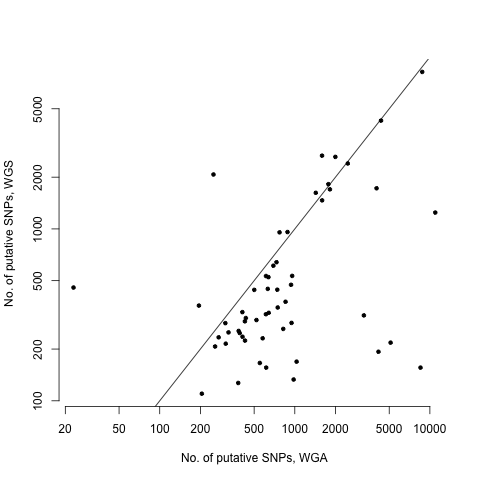
\includegraphics[scale=1.0]{C282_v_C484.png}
\caption{This figure plots the number of putative SNPs called by SomaticSniper (unfiltered) using the WGS v. WGA. Each point is a patient. The line is y=x, so points falling below the line agree with the hypothesis that whole genome amplification makes more mutations in a sample.}
\end{figure}

\begin{figure}
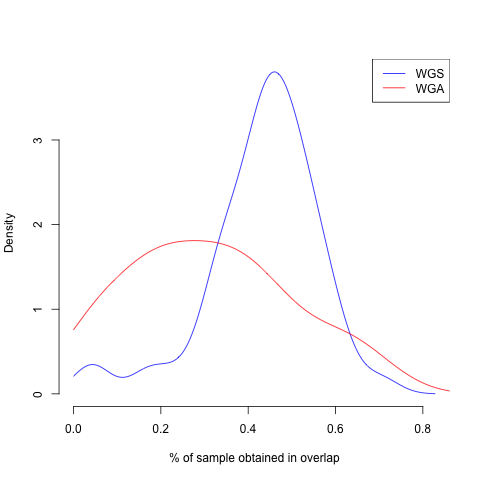
\includegraphics[scale=1.0]{unfiltered_overlap_WGS_WGA_together_densities.png}
\caption{This figure shows the density of the percentage of each WGS (blue) and WGA (red) sample that overlaps with the other sample from the same patient. The WGS distribution is higher and narrower, showing that the WGS samples overall have a higher percentage overlap than the WGA samples, and less range in this parameter. }
\end{figure}

\begin{figure}
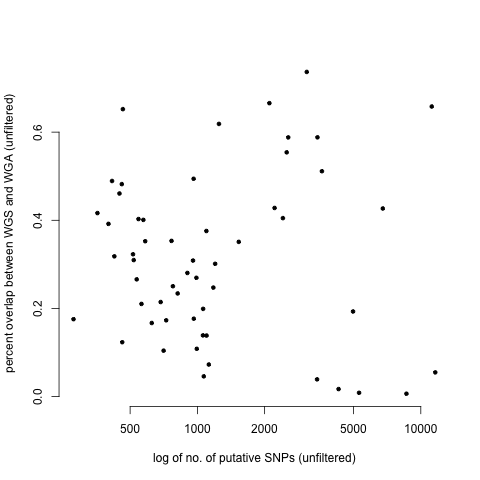
\includegraphics[scale=1.0]{unfiltered_total_muts_v_percent_overlap.png}
\caption{Plot of the percentage of the WGA samples that overlaped with the corresponding WGS samples (as a measure of sample quality) against the total number of putative SNPs in the WGS sample}
\end{figure}

\begin{figure}
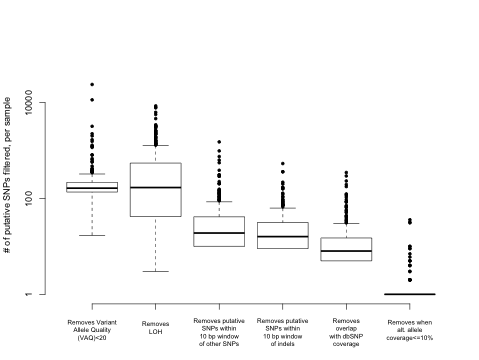
\includegraphics[scale=1.0]{boxplot_number_filtered.png}
\caption{Boxplot of the total number of putative SNPs removed by each of six filters, in each of 379 sequencing samples, from 311 patients. The x-axis gives the name of those filters that removed putative SNPs, and the y-axis gives, on a log scale, the number of mutations removed by a given sample.}
\end{figure}

\begin{figure}
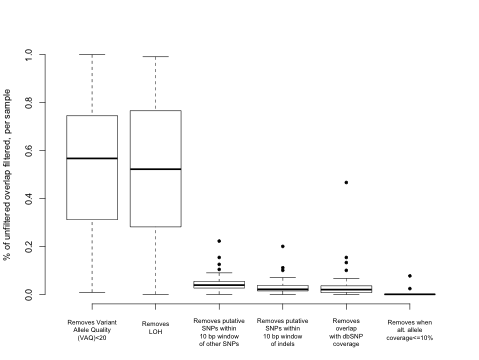
\includegraphics[scale=1.0]{boxplot_percent_overlap_filtered.png}
\caption{Boxplot of the percentage of putative SNPs making up the overlap between the WGS and WGA sequences of a single sample that was removed by a given filter. The x-axis describes the filters, and the y-axis gives the percentage of the overlap removed.}
\end{figure}

\bibliography{TCGA_bib}
\bibliographystyle{plain}

\end{document}

